\documentclass[1p]{elsarticle_modified}
%\bibliographystyle{elsarticle-num}

%\usepackage[colorlinks]{hyperref}
%\usepackage{abbrmath_seonhwa} %\Abb, \Ascr, \Acal ,\Abf, \Afrak
\usepackage{amsfonts}
\usepackage{amssymb}
\usepackage{amsmath}
\usepackage{amsthm}
\usepackage{scalefnt}
\usepackage{amsbsy}
\usepackage{kotex}
\usepackage{caption}
\usepackage{subfig}
\usepackage{color}
\usepackage{graphicx}
\usepackage{xcolor} %% white, black, red, green, blue, cyan, magenta, yellow
\usepackage{float}
\usepackage{setspace}
\usepackage{hyperref}

\usepackage{tikz}
\usetikzlibrary{arrows}

\usepackage{multirow}
\usepackage{array} % fixed length table
\usepackage{hhline}

%%%%%%%%%%%%%%%%%%%%%
\makeatletter
\renewcommand*\env@matrix[1][\arraystretch]{%
	\edef\arraystretch{#1}%
	\hskip -\arraycolsep
	\let\@ifnextchar\new@ifnextchar
	\array{*\c@MaxMatrixCols c}}
\makeatother %https://tex.stackexchange.com/questions/14071/how-can-i-increase-the-line-spacing-in-a-matrix
%%%%%%%%%%%%%%%

\usepackage[normalem]{ulem}

\newcommand{\msout}[1]{\ifmmode\text{\sout{\ensuremath{#1}}}\else\sout{#1}\fi}
%SOURCE: \msout is \stkout macro in https://tex.stackexchange.com/questions/20609/strikeout-in-math-mode

\newcommand{\cancel}[1]{
	\ifmmode
	{\color{red}\msout{#1}}
	\else
	{\color{red}\sout{#1}}
	\fi
}

\newcommand{\add}[1]{
	{\color{blue}\uwave{#1}}
}

\newcommand{\replace}[2]{
	\ifmmode
	{\color{red}\msout{#1}}{\color{blue}\uwave{#2}}
	\else
	{\color{red}\sout{#1}}{\color{blue}\uwave{#2}}
	\fi
}

\newcommand{\Sol}{\mathcal{S}} %segment
\newcommand{\D}{D} %diagram
\newcommand{\A}{\mathcal{A}} %arc


%%%%%%%%%%%%%%%%%%%%%%%%%%%%%5 test

\def\sl{\operatorname{\textup{SL}}(2,\Cbb)}
\def\psl{\operatorname{\textup{PSL}}(2,\Cbb)}
\def\quan{\mkern 1mu \triangleright \mkern 1mu}

\theoremstyle{definition}
\newtheorem{thm}{Theorem}[section]
\newtheorem{prop}[thm]{Proposition}
\newtheorem{lem}[thm]{Lemma}
\newtheorem{ques}[thm]{Question}
\newtheorem{cor}[thm]{Corollary}
\newtheorem{defn}[thm]{Definition}
\newtheorem{exam}[thm]{Example}
\newtheorem{rmk}[thm]{Remark}
\newtheorem{alg}[thm]{Algorithm}

\newcommand{\I}{\sqrt{-1}}
\begin{document}

%\begin{frontmatter}
%
%\title{Boundary parabolic representations of knots up to 8 crossings}
%
%%% Group authors per affiliation:
%\author{Yunhi Cho} 
%\address{Department of Mathematics, University of Seoul, Seoul, Korea}
%\ead{yhcho@uos.ac.kr}
%
%
%\author{Seonhwa Kim} %\fnref{s_kim}}
%\address{Center for Geometry and Physics, Institute for Basic Science, Pohang, 37673, Korea}
%\ead{ryeona17@ibs.re.kr}
%
%\author{Hyuk Kim}
%\address{Department of Mathematical Sciences, Seoul National University, Seoul 08826, Korea}
%\ead{hyukkim@snu.ac.kr}
%
%\author{Seokbeom Yoon}
%\address{Department of Mathematical Sciences, Seoul National University, Seoul, 08826,  Korea}
%\ead{sbyoon15@snu.ac.kr}
%
%\begin{abstract}
%We find all boundary parabolic representation of knots up to 8 crossings.
%
%\end{abstract}
%\begin{keyword}
%    \MSC[2010] 57M25 
%\end{keyword}
%
%\end{frontmatter}

%\linenumbers
%\tableofcontents
%
\newcommand\colored[1]{\textcolor{white}{\rule[-0.35ex]{0.8em}{1.4ex}}\kern-0.8em\color{red} #1}%
%\newcommand\colored[1]{\textcolor{white}{ #1}\kern-2.17ex	\textcolor{white}{ #1}\kern-1.81ex	\textcolor{white}{ #1}\kern-2.15ex\color{red}#1	}

{\Large $\underline{12n_{0127}~(K12n_{0127})}$}

\setlength{\tabcolsep}{10pt}
\renewcommand{\arraystretch}{1.6}
\vspace{1cm}\begin{tabular}{m{100pt}>{\centering\arraybackslash}m{274pt}}
\multirow{5}{120pt}{
	\centering
	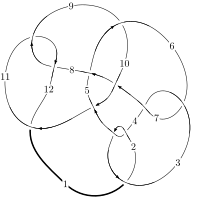
\includegraphics[width=112pt]{../../../GIT/diagram.site/Diagrams/png/2216_12n_0127.png}\\
\ \ \ A knot diagram\footnotemark}&
\allowdisplaybreaks
\textbf{Linearized knot diagam} \\
\cline{2-2}
 &
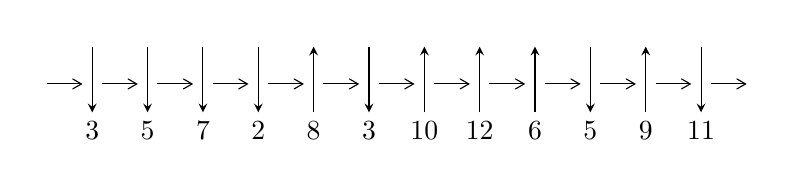
\begin{tikzpicture}[x=20pt, y=17pt]
	% nodes
	\node (C0) at (0, 0) {};
	\node (C1) at (1, 0) {};
	\node (C1U) at (1, +1) {};
	\node (C1D) at (1, -1) {3};

	\node (C2) at (2, 0) {};
	\node (C2U) at (2, +1) {};
	\node (C2D) at (2, -1) {5};

	\node (C3) at (3, 0) {};
	\node (C3U) at (3, +1) {};
	\node (C3D) at (3, -1) {7};

	\node (C4) at (4, 0) {};
	\node (C4U) at (4, +1) {};
	\node (C4D) at (4, -1) {2};

	\node (C5) at (5, 0) {};
	\node (C5U) at (5, +1) {};
	\node (C5D) at (5, -1) {8};

	\node (C6) at (6, 0) {};
	\node (C6U) at (6, +1) {};
	\node (C6D) at (6, -1) {3};

	\node (C7) at (7, 0) {};
	\node (C7U) at (7, +1) {};
	\node (C7D) at (7, -1) {10};

	\node (C8) at (8, 0) {};
	\node (C8U) at (8, +1) {};
	\node (C8D) at (8, -1) {12};

	\node (C9) at (9, 0) {};
	\node (C9U) at (9, +1) {};
	\node (C9D) at (9, -1) {6};

	\node (C10) at (10, 0) {};
	\node (C10U) at (10, +1) {};
	\node (C10D) at (10, -1) {5};

	\node (C11) at (11, 0) {};
	\node (C11U) at (11, +1) {};
	\node (C11D) at (11, -1) {9};

	\node (C12) at (12, 0) {};
	\node (C12U) at (12, +1) {};
	\node (C12D) at (12, -1) {11};
	\node (C13) at (13, 0) {};

	% arrows
	\draw[->,>={angle 60}]
	(C0) edge (C1) (C1) edge (C2) (C2) edge (C3) (C3) edge (C4) (C4) edge (C5) (C5) edge (C6) (C6) edge (C7) (C7) edge (C8) (C8) edge (C9) (C9) edge (C10) (C10) edge (C11) (C11) edge (C12) (C12) edge (C13) ;	\draw[->,>=stealth]
	(C1U) edge (C1D) (C2U) edge (C2D) (C3U) edge (C3D) (C4U) edge (C4D) (C5D) edge (C5U) (C6U) edge (C6D) (C7D) edge (C7U) (C8D) edge (C8U) (C9D) edge (C9U) (C10U) edge (C10D) (C11D) edge (C11U) (C12U) edge (C12D) ;
	\end{tikzpicture} \\
\hhline{~~} \\& 
\textbf{Solving Sequence} \\ \cline{2-2} 
 &
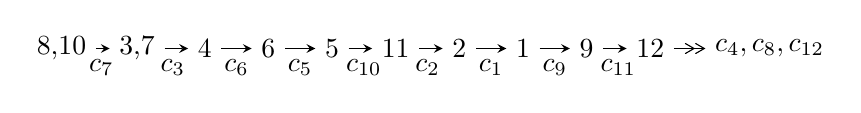
\begin{tikzpicture}[x=23pt, y=7pt]
	% node
	\node (A0) at (-1/8, 0) {8,10};
	\node (A1) at (17/16, 0) {3,7};
	\node (A2) at (17/8, 0) {4};
	\node (A3) at (25/8, 0) {6};
	\node (A4) at (33/8, 0) {5};
	\node (A5) at (41/8, 0) {11};
	\node (A6) at (49/8, 0) {2};
	\node (A7) at (57/8, 0) {1};
	\node (A8) at (65/8, 0) {9};
	\node (A9) at (73/8, 0) {12};
	\node (C1) at (1/2, -1) {$c_{7}$};
	\node (C2) at (13/8, -1) {$c_{3}$};
	\node (C3) at (21/8, -1) {$c_{6}$};
	\node (C4) at (29/8, -1) {$c_{5}$};
	\node (C5) at (37/8, -1) {$c_{10}$};
	\node (C6) at (45/8, -1) {$c_{2}$};
	\node (C7) at (53/8, -1) {$c_{1}$};
	\node (C8) at (61/8, -1) {$c_{9}$};
	\node (C9) at (69/8, -1) {$c_{11}$};
	\node (A10) at (11, 0) {$c_{4},c_{8},c_{12}$};

	% edge
	\draw[->,>=stealth]	
	(A0) edge (A1) (A1) edge (A2) (A2) edge (A3) (A3) edge (A4) (A4) edge (A5) (A5) edge (A6) (A6) edge (A7) (A7) edge (A8) (A8) edge (A9) ;
	\draw[->>,>={angle 60}]	
	(A9) edge (A10);
\end{tikzpicture} \\ 

\end{tabular} \\

\footnotetext{
The image of knot diagram is generated by the software ``\textbf{Draw programme}" developed by Andrew Bartholomew(\url{http://www.layer8.co.uk/maths/draw/index.htm\#Running-draw}), where we modified some parts for our purpose(\url{https://github.com/CATsTAILs/LinksPainter}).
}\phantom \\ \newline 
\centering \textbf{Ideals for irreducible components\footnotemark of $X_{\text{par}}$} 
 
\begin{align*}
I^u_{1}&=\langle 
5.41187\times10^{277} u^{67}-3.29717\times10^{278} u^{66}+\cdots+7.63032\times10^{279} b+2.06591\times10^{280},\\
\phantom{I^u_{1}}&\phantom{= \langle  }1.99190\times10^{278} u^{67}-1.24347\times10^{279} u^{66}+\cdots+1.41959\times10^{279} a+5.26734\times10^{280},\\
\phantom{I^u_{1}}&\phantom{= \langle  }u^{68}-6 u^{67}+\cdots+992 u+64\rangle \\
I^u_{2}&=\langle 
u^8-3 u^6+u^5+4 u^4-2 u^3- u^2+b+2 u-1,\;- u^8+2 u^7+2 u^6-5 u^5- u^4+5 u^3- u^2+a,\\
\phantom{I^u_{2}}&\phantom{= \langle  }u^9- u^8-2 u^7+3 u^6+u^5-3 u^4+2 u^3- u+1\rangle \\
\\
I^v_{1}&=\langle 
a,\;-186 v^5+1767 v^4-16759 v^3+279 v^2+385 b-93 v+306,\;v^6-10 v^5+95 v^4-48 v^3+15 v^2-5 v+1\rangle \\
\end{align*}
\raggedright * 3 irreducible components of $\dim_{\mathbb{C}}=0$, with total 83 representations.\\
\footnotetext{All coefficients of polynomials are rational numbers. But the coefficients are sometimes approximated in decimal forms when there is not enough margin.}
\newpage
\renewcommand{\arraystretch}{1}
\centering \section*{I. $I^u_{1}= \langle 5.41\times10^{277} u^{67}-3.30\times10^{278} u^{66}+\cdots+7.63\times10^{279} b+2.07\times10^{280},\;1.99\times10^{278} u^{67}-1.24\times10^{279} u^{66}+\cdots+1.42\times10^{279} a+5.27\times10^{280},\;u^{68}-6 u^{67}+\cdots+992 u+64 \rangle$}
\flushleft \textbf{(i) Arc colorings}\\
\begin{tabular}{m{7pt} m{180pt} m{7pt} m{180pt} }
\flushright $a_{8}=$&$\begin{pmatrix}1\\0\end{pmatrix}$ \\
\flushright $a_{10}=$&$\begin{pmatrix}0\\u\end{pmatrix}$ \\
\flushright $a_{3}=$&$\begin{pmatrix}-0.140315 u^{67}+0.875931 u^{66}+\cdots-399.413 u-37.1045\\-0.00709259 u^{67}+0.0432114 u^{66}+\cdots-24.8919 u-2.70750\end{pmatrix}$ \\
\flushright $a_{7}=$&$\begin{pmatrix}1\\u^2\end{pmatrix}$ \\
\flushright $a_{4}=$&$\begin{pmatrix}-0.140548 u^{67}+0.877681 u^{66}+\cdots-399.309 u-36.5756\\-0.00717314 u^{67}+0.0436428 u^{66}+\cdots-25.2257 u-2.73000\end{pmatrix}$ \\
\flushright $a_{6}=$&$\begin{pmatrix}-0.0867373 u^{67}+0.540807 u^{66}+\cdots-250.013 u-21.8923\\-0.00337015 u^{67}+0.0205084 u^{66}+\cdots-14.4347 u-1.57057\end{pmatrix}$ \\
\flushright $a_{5}=$&$\begin{pmatrix}-0.0833671 u^{67}+0.520298 u^{66}+\cdots-235.578 u-20.3217\\-0.00337015 u^{67}+0.0205084 u^{66}+\cdots-14.4347 u-1.57057\end{pmatrix}$ \\
\flushright $a_{11}=$&$\begin{pmatrix}-0.118608 u^{67}+0.755698 u^{66}+\cdots-203.655 u-6.99277\\-0.00539155 u^{67}+0.0336077 u^{66}+\cdots-12.9981 u-0.898136\end{pmatrix}$ \\
\flushright $a_{2}=$&$\begin{pmatrix}-0.0830107 u^{67}+0.517632 u^{66}+\cdots-243.251 u-23.6948\\-0.00363676 u^{67}+0.0222357 u^{66}+\cdots-13.9337 u-1.53678\end{pmatrix}$ \\
\flushright $a_{1}=$&$\begin{pmatrix}-0.0181153 u^{67}+0.110616 u^{66}+\cdots-71.0211 u-7.16788\\u^2\end{pmatrix}$ \\
\flushright $a_{9}=$&$\begin{pmatrix}-0.128840 u^{67}+0.819695 u^{66}+\cdots-230.862 u-8.73309\\-0.00484013 u^{67}+0.0303889 u^{66}+\cdots-12.2087 u-0.842183\end{pmatrix}$ \\
\flushright $a_{12}=$&$\begin{pmatrix}0.126251 u^{67}-0.763024 u^{66}+\cdots+580.255 u+57.9332\\0.000316220 u^{67}-0.00143516 u^{66}+\cdots+6.38612 u+0.783678\end{pmatrix}$\\&\end{tabular}
\flushleft \textbf{(ii) Obstruction class $= -1$}\\~\\
\flushleft \textbf{(iii) Cusp Shapes $= -0.416483 u^{67}+2.60331 u^{66}+\cdots-1160.89 u-97.1731$}\\~\\
\newpage\renewcommand{\arraystretch}{1}
\flushleft \textbf{(iv) u-Polynomials at the component}\newline \\
\begin{tabular}{m{50pt}|m{274pt}}
Crossings & \hspace{64pt}u-Polynomials at each crossing \\
\hline $$\begin{aligned}c_{1}\end{aligned}$$&$\begin{aligned}
&u^{68}+72 u^{67}+\cdots-116 u+1
\end{aligned}$\\
\hline $$\begin{aligned}c_{2},c_{4}\end{aligned}$$&$\begin{aligned}
&u^{68}-12 u^{67}+\cdots+4 u-1
\end{aligned}$\\
\hline $$\begin{aligned}c_{3},c_{6}\end{aligned}$$&$\begin{aligned}
&u^{68}+3 u^{67}+\cdots+2048 u+512
\end{aligned}$\\
\hline $$\begin{aligned}c_{5}\end{aligned}$$&$\begin{aligned}
&u^{68}+4 u^{67}+\cdots+20 u^2-1
\end{aligned}$\\
\hline $$\begin{aligned}c_{7}\end{aligned}$$&$\begin{aligned}
&u^{68}+6 u^{67}+\cdots-992 u+64
\end{aligned}$\\
\hline $$\begin{aligned}c_{8},c_{11}\end{aligned}$$&$\begin{aligned}
&u^{68}+5 u^{67}+\cdots-61 u+1
\end{aligned}$\\
\hline $$\begin{aligned}c_{9}\end{aligned}$$&$\begin{aligned}
&u^{68}-4 u^{67}+\cdots-1569175 u-179693
\end{aligned}$\\
\hline $$\begin{aligned}c_{10}\end{aligned}$$&$\begin{aligned}
&u^{68}-8 u^{67}+\cdots-679 u+1423
\end{aligned}$\\
\hline $$\begin{aligned}c_{12}\end{aligned}$$&$\begin{aligned}
&u^{68}+33 u^{67}+\cdots-4365 u+1
\end{aligned}$\\
\hline
\end{tabular}\\~\\
\newpage\renewcommand{\arraystretch}{1}
\flushleft \textbf{(v) Riley Polynomials at the component}\newline \\
\begin{tabular}{m{50pt}|m{274pt}}
Crossings & \hspace{64pt}Riley Polynomials at each crossing \\
\hline $$\begin{aligned}c_{1}\end{aligned}$$&$\begin{aligned}
&y^{68}-140 y^{67}+\cdots+13088 y+1
\end{aligned}$\\
\hline $$\begin{aligned}c_{2},c_{4}\end{aligned}$$&$\begin{aligned}
&y^{68}-72 y^{67}+\cdots+116 y+1
\end{aligned}$\\
\hline $$\begin{aligned}c_{3},c_{6}\end{aligned}$$&$\begin{aligned}
&y^{68}-51 y^{67}+\cdots-1048576 y+262144
\end{aligned}$\\
\hline $$\begin{aligned}c_{5}\end{aligned}$$&$\begin{aligned}
&y^{68}-16 y^{67}+\cdots-40 y+1
\end{aligned}$\\
\hline $$\begin{aligned}c_{7}\end{aligned}$$&$\begin{aligned}
&y^{68}+30 y^{67}+\cdots-332800 y+4096
\end{aligned}$\\
\hline $$\begin{aligned}c_{8},c_{11}\end{aligned}$$&$\begin{aligned}
&y^{68}+33 y^{67}+\cdots-4365 y+1
\end{aligned}$\\
\hline $$\begin{aligned}c_{9}\end{aligned}$$&$\begin{aligned}
&y^{68}-20 y^{67}+\cdots-70781434415 y+32289574249
\end{aligned}$\\
\hline $$\begin{aligned}c_{10}\end{aligned}$$&$\begin{aligned}
&y^{68}-68 y^{67}+\cdots+88237 y+2024929
\end{aligned}$\\
\hline $$\begin{aligned}c_{12}\end{aligned}$$&$\begin{aligned}
&y^{68}+9 y^{67}+\cdots-19115909 y+1
\end{aligned}$\\
\hline
\end{tabular}\\~\\
\newpage\flushleft \textbf{(vi) Complex Volumes and Cusp Shapes}
$$\begin{array}{c|c|c}  
\text{Solutions to }I^u_{1}& \I (\text{vol} + \sqrt{-1}CS) & \text{Cusp shape}\\
 \hline 
\begin{aligned}
u &= -0.950113 + 0.315579 I \\
a &= \phantom{-}0.548757 - 0.167876 I \\
b &= \phantom{-}0.776522 - 0.767567 I\end{aligned}
 & \phantom{-}1.45198 - 0.17538 I & \phantom{-0.000000 } 0 \\ \hline\begin{aligned}
u &= -0.950113 - 0.315579 I \\
a &= \phantom{-}0.548757 + 0.167876 I \\
b &= \phantom{-}0.776522 + 0.767567 I\end{aligned}
 & \phantom{-}1.45198 + 0.17538 I & \phantom{-0.000000 } 0 \\ \hline\begin{aligned}
u &= -0.138014 + 0.941313 I \\
a &= -1.52735 - 0.38576 I \\
b &= -0.026016 + 0.803652 I\end{aligned}
 & -1.98118 - 0.16998 I & \phantom{-0.000000 } 0 \\ \hline\begin{aligned}
u &= -0.138014 - 0.941313 I \\
a &= -1.52735 + 0.38576 I \\
b &= -0.026016 - 0.803652 I\end{aligned}
 & -1.98118 + 0.16998 I & \phantom{-0.000000 } 0 \\ \hline\begin{aligned}
u &= -0.985804 + 0.387544 I \\
a &= \phantom{-}0.0078436 - 0.0769643 I \\
b &= -0.113466 - 0.711289 I\end{aligned}
 & \phantom{-}3.23957 - 1.57241 I & \phantom{-0.000000 } 0 \\ \hline\begin{aligned}
u &= -0.985804 - 0.387544 I \\
a &= \phantom{-}0.0078436 + 0.0769643 I \\
b &= -0.113466 + 0.711289 I\end{aligned}
 & \phantom{-}3.23957 + 1.57241 I & \phantom{-0.000000 } 0 \\ \hline\begin{aligned}
u &= \phantom{-}0.654795 + 0.664515 I \\
a &= -0.052917 - 0.398943 I \\
b &= \phantom{-}0.109744 + 0.545343 I\end{aligned}
 & -1.99133 + 1.66625 I & \phantom{-0.000000 } 0. - 3.30828 I \\ \hline\begin{aligned}
u &= \phantom{-}0.654795 - 0.664515 I \\
a &= -0.052917 + 0.398943 I \\
b &= \phantom{-}0.109744 - 0.545343 I\end{aligned}
 & -1.99133 - 1.66625 I & \phantom{-0.000000 -}0. + 3.30828 I \\ \hline\begin{aligned}
u &= \phantom{-}0.918521 + 0.022770 I \\
a &= -0.80746 - 3.11284 I \\
b &= -0.45158 - 1.99901 I\end{aligned}
 & -2.78363 - 2.76140 I & \phantom{-0.000000 -}0. + 6.78295 I \\ \hline\begin{aligned}
u &= \phantom{-}0.918521 - 0.022770 I \\
a &= -0.80746 + 3.11284 I \\
b &= -0.45158 + 1.99901 I\end{aligned}
 & -2.78363 + 2.76140 I & \phantom{-0.000000 } 0. - 6.78295 I\\
 \hline 
 \end{array}$$\newpage$$\begin{array}{c|c|c}  
\text{Solutions to }I^u_{1}& \I (\text{vol} + \sqrt{-1}CS) & \text{Cusp shape}\\
 \hline 
\begin{aligned}
u &= \phantom{-}0.618022 + 0.678734 I \\
a &= \phantom{-}0.34805 + 1.72657 I \\
b &= -0.0123186 + 0.1252700 I\end{aligned}
 & -7.66872 + 1.43842 I & -12.36030 + 0. I\phantom{ +0.000000I} \\ \hline\begin{aligned}
u &= \phantom{-}0.618022 - 0.678734 I \\
a &= \phantom{-}0.34805 - 1.72657 I \\
b &= -0.0123186 - 0.1252700 I\end{aligned}
 & -7.66872 - 1.43842 I & -12.36030 + 0. I\phantom{ +0.000000I} \\ \hline\begin{aligned}
u &= -0.833182 + 0.382913 I \\
a &= -1.22956 - 1.32718 I \\
b &= \phantom{-}0.0823456 - 0.0914731 I\end{aligned}
 & -9.13954 + 3.03771 I & -6.42466 + 6.40081 I \\ \hline\begin{aligned}
u &= -0.833182 - 0.382913 I \\
a &= -1.22956 + 1.32718 I \\
b &= \phantom{-}0.0823456 + 0.0914731 I\end{aligned}
 & -9.13954 - 3.03771 I & -6.42466 - 6.40081 I \\ \hline\begin{aligned}
u &= -0.343117 + 1.102390 I \\
a &= \phantom{-}1.62260 + 0.06591 I \\
b &= -1.11538 - 1.08043 I\end{aligned}
 & \phantom{-}1.02080 - 2.73193 I & \phantom{-0.000000 } 0 \\ \hline\begin{aligned}
u &= -0.343117 - 1.102390 I \\
a &= \phantom{-}1.62260 - 0.06591 I \\
b &= -1.11538 + 1.08043 I\end{aligned}
 & \phantom{-}1.02080 + 2.73193 I & \phantom{-0.000000 } 0 \\ \hline\begin{aligned}
u &= -0.091668 + 1.182840 I \\
a &= -1.058340 + 0.288071 I \\
b &= \phantom{-}0.110946 - 0.754708 I\end{aligned}
 & -5.18749 - 3.49319 I & \phantom{-0.000000 } 0 \\ \hline\begin{aligned}
u &= -0.091668 - 1.182840 I \\
a &= -1.058340 - 0.288071 I \\
b &= \phantom{-}0.110946 + 0.754708 I\end{aligned}
 & -5.18749 + 3.49319 I & \phantom{-0.000000 } 0 \\ \hline\begin{aligned}
u &= \phantom{-}1.058570 + 0.536792 I \\
a &= -0.0374936 + 0.0394319 I \\
b &= -0.072006 + 0.563424 I\end{aligned}
 & \phantom{-}2.39963 + 7.06465 I & \phantom{-0.000000 } 0 \\ \hline\begin{aligned}
u &= \phantom{-}1.058570 - 0.536792 I \\
a &= -0.0374936 - 0.0394319 I \\
b &= -0.072006 - 0.563424 I\end{aligned}
 & \phantom{-}2.39963 - 7.06465 I & \phantom{-0.000000 } 0\\
 \hline 
 \end{array}$$\newpage$$\begin{array}{c|c|c}  
\text{Solutions to }I^u_{1}& \I (\text{vol} + \sqrt{-1}CS) & \text{Cusp shape}\\
 \hline 
\begin{aligned}
u &= \phantom{-}0.291235 + 0.741989 I \\
a &= \phantom{-}1.43685 - 0.21711 I \\
b &= -0.423071 + 0.457603 I\end{aligned}
 & \phantom{-}0.59153 - 2.55241 I & \phantom{-}2.37006 + 1.53670 I \\ \hline\begin{aligned}
u &= \phantom{-}0.291235 - 0.741989 I \\
a &= \phantom{-}1.43685 + 0.21711 I \\
b &= -0.423071 - 0.457603 I\end{aligned}
 & \phantom{-}0.59153 + 2.55241 I & \phantom{-}2.37006 - 1.53670 I \\ \hline\begin{aligned}
u &= \phantom{-}0.284392 + 1.184020 I \\
a &= -1.348990 + 0.014290 I \\
b &= \phantom{-}0.066230 - 0.901010 I\end{aligned}
 & -4.78405 + 4.34186 I & \phantom{-0.000000 } 0 \\ \hline\begin{aligned}
u &= \phantom{-}0.284392 - 1.184020 I \\
a &= -1.348990 - 0.014290 I \\
b &= \phantom{-}0.066230 + 0.901010 I\end{aligned}
 & -4.78405 - 4.34186 I & \phantom{-0.000000 } 0 \\ \hline\begin{aligned}
u &= -0.378527 + 1.199800 I \\
a &= -0.185821 - 0.027577 I \\
b &= \phantom{-}0.08329 + 1.60214 I\end{aligned}
 & -3.90942 - 3.06813 I & \phantom{-0.000000 } 0 \\ \hline\begin{aligned}
u &= -0.378527 - 1.199800 I \\
a &= -0.185821 + 0.027577 I \\
b &= \phantom{-}0.08329 - 1.60214 I\end{aligned}
 & -3.90942 + 3.06813 I & \phantom{-0.000000 } 0 \\ \hline\begin{aligned}
u &= \phantom{-}0.618286 + 1.143470 I \\
a &= \phantom{-}0.941109 + 0.552542 I \\
b &= -0.161234 + 0.197997 I\end{aligned}
 & -9.06891 + 3.72651 I & \phantom{-0.000000 } 0 \\ \hline\begin{aligned}
u &= \phantom{-}0.618286 - 1.143470 I \\
a &= \phantom{-}0.941109 - 0.552542 I \\
b &= -0.161234 - 0.197997 I\end{aligned}
 & -9.06891 - 3.72651 I & \phantom{-0.000000 } 0 \\ \hline\begin{aligned}
u &= \phantom{-}1.215690 + 0.466052 I \\
a &= \phantom{-}0.729712 + 0.700660 I \\
b &= \phantom{-}0.98247 + 1.78974 I\end{aligned}
 & -1.26231 - 4.39904 I & \phantom{-0.000000 } 0 \\ \hline\begin{aligned}
u &= \phantom{-}1.215690 - 0.466052 I \\
a &= \phantom{-}0.729712 - 0.700660 I \\
b &= \phantom{-}0.98247 - 1.78974 I\end{aligned}
 & -1.26231 + 4.39904 I & \phantom{-0.000000 } 0\\
 \hline 
 \end{array}$$\newpage$$\begin{array}{c|c|c}  
\text{Solutions to }I^u_{1}& \I (\text{vol} + \sqrt{-1}CS) & \text{Cusp shape}\\
 \hline 
\begin{aligned}
u &= -0.533248 + 0.422514 I \\
a &= -3.12926 + 0.99004 I \\
b &= -0.520884 + 1.056390 I\end{aligned}
 & -1.175210 - 0.433161 I & -4.73090 + 4.14534 I \\ \hline\begin{aligned}
u &= -0.533248 - 0.422514 I \\
a &= -3.12926 - 0.99004 I \\
b &= -0.520884 - 1.056390 I\end{aligned}
 & -1.175210 + 0.433161 I & -4.73090 - 4.14534 I \\ \hline\begin{aligned}
u &= -0.395435 + 1.259920 I \\
a &= \phantom{-}1.202320 - 0.400059 I \\
b &= -0.210830 - 0.120552 I\end{aligned}
 & -13.78770 - 0.65730 I & \phantom{-0.000000 } 0 \\ \hline\begin{aligned}
u &= -0.395435 - 1.259920 I \\
a &= \phantom{-}1.202320 + 0.400059 I \\
b &= -0.210830 + 0.120552 I\end{aligned}
 & -13.78770 + 0.65730 I & \phantom{-0.000000 } 0 \\ \hline\begin{aligned}
u &= \phantom{-}0.195281 + 1.367220 I \\
a &= \phantom{-}0.161197 + 0.187003 I \\
b &= -0.03055 - 1.73074 I\end{aligned}
 & -8.15277 - 0.56922 I & \phantom{-0.000000 } 0 \\ \hline\begin{aligned}
u &= \phantom{-}0.195281 - 1.367220 I \\
a &= \phantom{-}0.161197 - 0.187003 I \\
b &= -0.03055 + 1.73074 I\end{aligned}
 & -8.15277 + 0.56922 I & \phantom{-0.000000 } 0 \\ \hline\begin{aligned}
u &= \phantom{-}0.501266 + 1.311640 I \\
a &= -0.032263 - 0.145766 I \\
b &= -0.00664 - 1.54510 I\end{aligned}
 & -6.75213 + 7.96693 I & \phantom{-0.000000 } 0 \\ \hline\begin{aligned}
u &= \phantom{-}0.501266 - 1.311640 I \\
a &= -0.032263 + 0.145766 I \\
b &= -0.00664 + 1.54510 I\end{aligned}
 & -6.75213 - 7.96693 I & \phantom{-0.000000 } 0 \\ \hline\begin{aligned}
u &= -0.651697 + 1.252300 I \\
a &= \phantom{-}1.368070 - 0.194338 I \\
b &= -0.50799 - 1.66891 I\end{aligned}
 & -1.42714 - 5.94125 I & \phantom{-0.000000 } 0 \\ \hline\begin{aligned}
u &= -0.651697 - 1.252300 I \\
a &= \phantom{-}1.368070 + 0.194338 I \\
b &= -0.50799 + 1.66891 I\end{aligned}
 & -1.42714 + 5.94125 I & \phantom{-0.000000 } 0\\
 \hline 
 \end{array}$$\newpage$$\begin{array}{c|c|c}  
\text{Solutions to }I^u_{1}& \I (\text{vol} + \sqrt{-1}CS) & \text{Cusp shape}\\
 \hline 
\begin{aligned}
u &= -0.443948 + 0.381193 I \\
a &= \phantom{-}0.023452 - 0.289831 I \\
b &= -0.092531 - 1.256890 I\end{aligned}
 & \phantom{-}3.20421 - 1.15270 I & \phantom{-}2.54366 + 10.12386 I \\ \hline\begin{aligned}
u &= -0.443948 - 0.381193 I \\
a &= \phantom{-}0.023452 + 0.289831 I \\
b &= -0.092531 + 1.256890 I\end{aligned}
 & \phantom{-}3.20421 + 1.15270 I & \phantom{-}2.54366 - 10.12386 I \\ \hline\begin{aligned}
u &= -0.68544 + 1.24203 I \\
a &= \phantom{-}0.920678 - 0.419746 I \\
b &= -0.202383 - 0.229028 I\end{aligned}
 & -11.5445 - 8.9372 I & \phantom{-0.000000 } 0 \\ \hline\begin{aligned}
u &= -0.68544 - 1.24203 I \\
a &= \phantom{-}0.920678 + 0.419746 I \\
b &= -0.202383 + 0.229028 I\end{aligned}
 & -11.5445 + 8.9372 I & \phantom{-0.000000 } 0 \\ \hline\begin{aligned}
u &= -0.047717 + 0.545973 I \\
a &= -0.040233 + 0.322065 I \\
b &= -0.19956 + 1.40398 I\end{aligned}
 & \phantom{-}2.67134 + 4.86258 I & -14.4423 - 3.8383 I \\ \hline\begin{aligned}
u &= -0.047717 - 0.545973 I \\
a &= -0.040233 - 0.322065 I \\
b &= -0.19956 - 1.40398 I\end{aligned}
 & \phantom{-}2.67134 - 4.86258 I & -14.4423 + 3.8383 I \\ \hline\begin{aligned}
u &= \phantom{-}0.53438 + 1.35483 I \\
a &= \phantom{-}1.200600 + 0.014989 I \\
b &= -0.49203 + 1.82310 I\end{aligned}
 & -6.53057 + 2.65488 I & \phantom{-0.000000 } 0 \\ \hline\begin{aligned}
u &= \phantom{-}0.53438 - 1.35483 I \\
a &= \phantom{-}1.200600 - 0.014989 I \\
b &= -0.49203 - 1.82310 I\end{aligned}
 & -6.53057 - 2.65488 I & \phantom{-0.000000 } 0 \\ \hline\begin{aligned}
u &= \phantom{-}0.477410 + 0.194259 I \\
a &= \phantom{-}3.46449 - 0.24479 I \\
b &= \phantom{-}0.066672 + 0.494530 I\end{aligned}
 & -1.07758 + 1.62874 I & \phantom{-}1.55460 - 6.14952 I \\ \hline\begin{aligned}
u &= \phantom{-}0.477410 - 0.194259 I \\
a &= \phantom{-}3.46449 + 0.24479 I \\
b &= \phantom{-}0.066672 - 0.494530 I\end{aligned}
 & -1.07758 - 1.62874 I & \phantom{-}1.55460 + 6.14952 I\\
 \hline 
 \end{array}$$\newpage$$\begin{array}{c|c|c}  
\text{Solutions to }I^u_{1}& \I (\text{vol} + \sqrt{-1}CS) & \text{Cusp shape}\\
 \hline 
\begin{aligned}
u &= \phantom{-}0.72857 + 1.29465 I \\
a &= \phantom{-}1.294820 + 0.292927 I \\
b &= -0.44191 + 1.67576 I\end{aligned}
 & -4.00028 + 11.30660 I & \phantom{-0.000000 } 0 \\ \hline\begin{aligned}
u &= \phantom{-}0.72857 - 1.29465 I \\
a &= \phantom{-}1.294820 - 0.292927 I \\
b &= -0.44191 - 1.67576 I\end{aligned}
 & -4.00028 - 11.30660 I & \phantom{-0.000000 } 0 \\ \hline\begin{aligned}
u &= -0.199150 + 0.463613 I \\
a &= -5.65825 + 2.26682 I \\
b &= \phantom{-}0.979716 + 0.919145 I\end{aligned}
 & -1.11507 - 2.15821 I & -17.5757 + 1.3433 I \\ \hline\begin{aligned}
u &= -0.199150 - 0.463613 I \\
a &= -5.65825 - 2.26682 I \\
b &= \phantom{-}0.979716 - 0.919145 I\end{aligned}
 & -1.11507 + 2.15821 I & -17.5757 - 1.3433 I \\ \hline\begin{aligned}
u &= -0.207672 + 0.089139 I \\
a &= \phantom{-}11.0630 + 18.1211 I \\
b &= \phantom{-}0.455149 + 0.270879 I\end{aligned}
 & -1.10951 - 2.08005 I & \phantom{-}43.7323 + 52.4587 I \\ \hline\begin{aligned}
u &= -0.207672 - 0.089139 I \\
a &= \phantom{-}11.0630 - 18.1211 I \\
b &= \phantom{-}0.455149 - 0.270879 I\end{aligned}
 & -1.10951 + 2.08005 I & \phantom{-}43.7323 - 52.4587 I \\ \hline\begin{aligned}
u &= \phantom{-}1.06862 + 1.46334 I \\
a &= -1.083940 - 0.489279 I \\
b &= \phantom{-}1.02549 - 2.05791 I\end{aligned}
 & -10.9823 + 16.7933 I & \phantom{-0.000000 } 0 \\ \hline\begin{aligned}
u &= \phantom{-}1.06862 - 1.46334 I \\
a &= -1.083940 + 0.489279 I \\
b &= \phantom{-}1.02549 + 2.05791 I\end{aligned}
 & -10.9823 - 16.7933 I & \phantom{-0.000000 } 0 \\ \hline\begin{aligned}
u &= -1.00127 + 1.57480 I \\
a &= -1.057930 + 0.383092 I \\
b &= \phantom{-}1.22819 + 2.06366 I\end{aligned}
 & -8.36607 - 10.64720 I & \phantom{-0.000000 } 0 \\ \hline\begin{aligned}
u &= -1.00127 - 1.57480 I \\
a &= -1.057930 - 0.383092 I \\
b &= \phantom{-}1.22819 - 2.06366 I\end{aligned}
 & -8.36607 + 10.64720 I & \phantom{-0.000000 } 0\\
 \hline 
 \end{array}$$\newpage$$\begin{array}{c|c|c}  
\text{Solutions to }I^u_{1}& \I (\text{vol} + \sqrt{-1}CS) & \text{Cusp shape}\\
 \hline 
\begin{aligned}
u &= -0.122992\phantom{ +0.000000I} \\
a &= -7.00758\phantom{ +0.000000I} \\
b &= -0.657961\phantom{ +0.000000I}\end{aligned}
 & -1.12640\phantom{ +0.000000I} & -9.50710\phantom{ +0.000000I} \\ \hline\begin{aligned}
u &= \phantom{-}1.18225 + 1.81842 I \\
a &= -0.873443 - 0.339937 I \\
b &= \phantom{-}1.41202 - 2.62610 I\end{aligned}
 & -14.9486 + 6.6050 I & \phantom{-0.000000 } 0 \\ \hline\begin{aligned}
u &= \phantom{-}1.18225 - 1.81842 I \\
a &= -0.873443 + 0.339937 I \\
b &= \phantom{-}1.41202 + 2.62610 I\end{aligned}
 & -14.9486 - 6.6050 I & \phantom{-0.000000 } 0 \\ \hline\begin{aligned}
u &= \phantom{-}2.21003 + 0.87540 I \\
a &= -0.404299 - 0.141048 I \\
b &= -2.64545 - 2.40849 I\end{aligned}
 & -8.52431 - 6.48393 I & \phantom{-0.000000 } 0 \\ \hline\begin{aligned}
u &= \phantom{-}2.21003 - 0.87540 I \\
a &= -0.404299 + 0.141048 I \\
b &= -2.64545 + 2.40849 I\end{aligned}
 & -8.52431 + 6.48393 I & \phantom{-0.000000 } 0 \\ \hline\begin{aligned}
u &= -2.40291\phantom{ +0.000000I} \\
a &= -0.382796\phantom{ +0.000000I} \\
b &= -3.59332\phantom{ +0.000000I}\end{aligned}
 & -4.25382\phantom{ +0.000000I} & \phantom{-0.000000 } 0 \\ \hline\begin{aligned}
u &= -0.40837 + 2.39079 I \\
a &= -0.860811 + 0.059303 I \\
b &= \phantom{-}3.47268 + 1.22842 I\end{aligned}
 & -5.26056 - 3.80306 I & \phantom{-0.000000 } 0 \\ \hline\begin{aligned}
u &= -0.40837 - 2.39079 I \\
a &= -0.860811 - 0.059303 I \\
b &= \phantom{-}3.47268 - 1.22842 I\end{aligned}
 & -5.26056 + 3.80306 I & \phantom{-0.000000 } 0\\
 \hline 
 \end{array}$$\newpage\newpage\renewcommand{\arraystretch}{1}
\centering \section*{II. $I^u_{2}= \langle u^8-3 u^6+u^5+4 u^4-2 u^3- u^2+b+2 u-1,\;- u^8+2 u^7+2 u^6-5 u^5- u^4+5 u^3- u^2+a,\;u^9- u^8-2 u^7+3 u^6+u^5-3 u^4+2 u^3- u+1 \rangle$}
\flushleft \textbf{(i) Arc colorings}\\
\begin{tabular}{m{7pt} m{180pt} m{7pt} m{180pt} }
\flushright $a_{8}=$&$\begin{pmatrix}1\\0\end{pmatrix}$ \\
\flushright $a_{10}=$&$\begin{pmatrix}0\\u\end{pmatrix}$ \\
\flushright $a_{3}=$&$\begin{pmatrix}u^8-2 u^7-2 u^6+5 u^5+u^4-5 u^3+u^2\\- u^8+3 u^6- u^5-4 u^4+2 u^3+u^2-2 u+1\end{pmatrix}$ \\
\flushright $a_{7}=$&$\begin{pmatrix}1\\u^2\end{pmatrix}$ \\
\flushright $a_{4}=$&$\begin{pmatrix}u^8-2 u^7-2 u^6+5 u^5+u^4-5 u^3+u^2\\- u^8+3 u^6- u^5-4 u^4+2 u^3+u^2-2 u+1\end{pmatrix}$ \\
\flushright $a_{6}=$&$\begin{pmatrix}1\\u^2\end{pmatrix}$ \\
\flushright $a_{5}=$&$\begin{pmatrix}- u^2+1\\u^2\end{pmatrix}$ \\
\flushright $a_{11}=$&$\begin{pmatrix}- u^5+2 u^3- u\\u^5- u^3+u\end{pmatrix}$ \\
\flushright $a_{2}=$&$\begin{pmatrix}u^8-2 u^7-2 u^6+5 u^5+u^4-5 u^3+2 u^2-1\\- u^8+3 u^6- u^5-4 u^4+2 u^3-2 u+1\end{pmatrix}$ \\
\flushright $a_{1}=$&$\begin{pmatrix}u^2-1\\- u^2\end{pmatrix}$ \\
\flushright $a_{9}=$&$\begin{pmatrix}- u\\- u^3+u\end{pmatrix}$ \\
\flushright $a_{12}=$&$\begin{pmatrix}u^8-3 u^6+3 u^4-1\\- u^8+2 u^6-2 u^4\end{pmatrix}$\\&\end{tabular}
\flushleft \textbf{(ii) Obstruction class $= 1$}\\~\\
\flushleft \textbf{(iii) Cusp Shapes $= 5 u^8-9 u^7-7 u^6+22 u^5-2 u^4-23 u^3+13 u^2- u-9$}\\~\\
\newpage\renewcommand{\arraystretch}{1}
\flushleft \textbf{(iv) u-Polynomials at the component}\newline \\
\begin{tabular}{m{50pt}|m{274pt}}
Crossings & \hspace{64pt}u-Polynomials at each crossing \\
\hline $$\begin{aligned}c_{1},c_{2}\end{aligned}$$&$\begin{aligned}
&(u-1)^9
\end{aligned}$\\
\hline $$\begin{aligned}c_{3},c_{6}\end{aligned}$$&$\begin{aligned}
&u^9
\end{aligned}$\\
\hline $$\begin{aligned}c_{4}\end{aligned}$$&$\begin{aligned}
&(u+1)^9
\end{aligned}$\\
\hline $$\begin{aligned}c_{5}\end{aligned}$$&$\begin{aligned}
&u^9+5 u^8+12 u^7+15 u^6+9 u^5- u^4-4 u^3-2 u^2+u+1
\end{aligned}$\\
\hline $$\begin{aligned}c_{7}\end{aligned}$$&$\begin{aligned}
&u^9- u^8-2 u^7+3 u^6+u^5-3 u^4+2 u^3- u+1
\end{aligned}$\\
\hline $$\begin{aligned}c_{8}\end{aligned}$$&$\begin{aligned}
&u^9- u^8+2 u^7- u^6+3 u^5- u^4+2 u^3+u+1
\end{aligned}$\\
\hline $$\begin{aligned}c_{9}\end{aligned}$$&$\begin{aligned}
&u^9+u^8-2 u^7-3 u^6+u^5+3 u^4+2 u^3- u-1
\end{aligned}$\\
\hline $$\begin{aligned}c_{10},c_{12}\end{aligned}$$&$\begin{aligned}
&u^9+3 u^8+8 u^7+13 u^6+17 u^5+17 u^4+12 u^3+6 u^2+u-1
\end{aligned}$\\
\hline $$\begin{aligned}c_{11}\end{aligned}$$&$\begin{aligned}
&u^9+u^8+2 u^7+u^6+3 u^5+u^4+2 u^3+u-1
\end{aligned}$\\
\hline
\end{tabular}\\~\\
\newpage\renewcommand{\arraystretch}{1}
\flushleft \textbf{(v) Riley Polynomials at the component}\newline \\
\begin{tabular}{m{50pt}|m{274pt}}
Crossings & \hspace{64pt}Riley Polynomials at each crossing \\
\hline $$\begin{aligned}c_{1},c_{2},c_{4}\end{aligned}$$&$\begin{aligned}
&(y-1)^9
\end{aligned}$\\
\hline $$\begin{aligned}c_{3},c_{6}\end{aligned}$$&$\begin{aligned}
&y^9
\end{aligned}$\\
\hline $$\begin{aligned}c_{5}\end{aligned}$$&$\begin{aligned}
&y^9- y^8+12 y^7-7 y^6+37 y^5+y^4-10 y^2+5 y-1
\end{aligned}$\\
\hline $$\begin{aligned}c_{7},c_{9}\end{aligned}$$&$\begin{aligned}
&y^9-5 y^8+12 y^7-15 y^6+9 y^5+y^4-4 y^3+2 y^2+y-1
\end{aligned}$\\
\hline $$\begin{aligned}c_{8},c_{11}\end{aligned}$$&$\begin{aligned}
&y^9+3 y^8+8 y^7+13 y^6+17 y^5+17 y^4+12 y^3+6 y^2+y-1
\end{aligned}$\\
\hline $$\begin{aligned}c_{10},c_{12}\end{aligned}$$&$\begin{aligned}
&y^9+7 y^8+20 y^7+25 y^6+5 y^5-15 y^4+22 y^2+13 y-1
\end{aligned}$\\
\hline
\end{tabular}\\~\\
\newpage\flushleft \textbf{(vi) Complex Volumes and Cusp Shapes}
$$\begin{array}{c|c|c}  
\text{Solutions to }I^u_{2}& \I (\text{vol} + \sqrt{-1}CS) & \text{Cusp shape}\\
 \hline 
\begin{aligned}
u &= \phantom{-}0.772920 + 0.510351 I \\
a &= -0.939568 - 0.981640 I \\
b &= \phantom{-}0.457852 - 1.072010 I\end{aligned}
 & -3.42837 + 2.09337 I & -8.61953 - 2.85927 I \\ \hline\begin{aligned}
u &= \phantom{-}0.772920 - 0.510351 I \\
a &= -0.939568 + 0.981640 I \\
b &= \phantom{-}0.457852 + 1.072010 I\end{aligned}
 & -3.42837 - 2.09337 I & -8.61953 + 2.85927 I \\ \hline\begin{aligned}
u &= -0.825933\phantom{ +0.000000I} \\
a &= \phantom{-}2.14893\phantom{ +0.000000I} \\
b &= \phantom{-}1.46592\phantom{ +0.000000I}\end{aligned}
 & -0.446489\phantom{ +0.000000I} & \phantom{-}5.48680\phantom{ +0.000000I} \\ \hline\begin{aligned}
u &= -1.173910 + 0.391555 I \\
a &= \phantom{-}0.119081 + 0.409451 I \\
b &= \phantom{-}0.522253 + 0.392004 I\end{aligned}
 & \phantom{-}2.72642 - 1.33617 I & -5.51122 - 2.15019 I \\ \hline\begin{aligned}
u &= -1.173910 - 0.391555 I \\
a &= \phantom{-}0.119081 - 0.409451 I \\
b &= \phantom{-}0.522253 - 0.392004 I\end{aligned}
 & \phantom{-}2.72642 + 1.33617 I & -5.51122 + 2.15019 I \\ \hline\begin{aligned}
u &= \phantom{-}0.141484 + 0.739668 I \\
a &= \phantom{-}2.26219 + 2.13290 I \\
b &= -1.63880 - 0.65075 I\end{aligned}
 & -1.02799 - 2.45442 I & -5.09778 + 12.45976 I \\ \hline\begin{aligned}
u &= \phantom{-}0.141484 - 0.739668 I \\
a &= \phantom{-}2.26219 - 2.13290 I \\
b &= -1.63880 + 0.65075 I\end{aligned}
 & -1.02799 + 2.45442 I & -5.09778 - 12.45976 I \\ \hline\begin{aligned}
u &= \phantom{-}1.172470 + 0.500383 I \\
a &= -0.016164 - 0.378317 I \\
b &= \phantom{-}0.425734 - 0.444312 I\end{aligned}
 & \phantom{-}1.95319 + 7.08493 I & -9.51486 - 6.49599 I \\ \hline\begin{aligned}
u &= \phantom{-}1.172470 - 0.500383 I \\
a &= -0.016164 + 0.378317 I \\
b &= \phantom{-}0.425734 + 0.444312 I\end{aligned}
 & \phantom{-}1.95319 - 7.08493 I & -9.51486 + 6.49599 I\\
 \hline 
 \end{array}$$\newpage\newpage\renewcommand{\arraystretch}{1}
\centering \section*{III. $I^v_{1}= \langle a,\;-186 v^5+1767 v^4+\cdots+385 b+306,\;v^6-10 v^5+95 v^4-48 v^3+15 v^2-5 v+1 \rangle$}
\flushleft \textbf{(i) Arc colorings}\\
\begin{tabular}{m{7pt} m{180pt} m{7pt} m{180pt} }
\flushright $a_{8}=$&$\begin{pmatrix}1\\0\end{pmatrix}$ \\
\flushright $a_{10}=$&$\begin{pmatrix}v\\0\end{pmatrix}$ \\
\flushright $a_{3}=$&$\begin{pmatrix}0\\0.483117 v^{5}-4.58961 v^{4}+\cdots+0.241558 v-0.794805\end{pmatrix}$ \\
\flushright $a_{7}=$&$\begin{pmatrix}1\\0\end{pmatrix}$ \\
\flushright $a_{4}=$&$\begin{pmatrix}-0.483117 v^{5}+4.58961 v^{4}+\cdots-0.241558 v+0.794805\\0.483117 v^{5}-4.58961 v^{4}+\cdots+0.241558 v-0.794805\end{pmatrix}$ \\
\flushright $a_{6}=$&$\begin{pmatrix}1\\0.207792 v^{5}-1.97403 v^{4}+\cdots+0.103896 v+1.41299\end{pmatrix}$ \\
\flushright $a_{5}=$&$\begin{pmatrix}-0.207792 v^{5}+1.97403 v^{4}+\cdots-0.103896 v-0.412987\\0.207792 v^{5}-1.97403 v^{4}+\cdots+0.103896 v+1.41299\end{pmatrix}$ \\
\flushright $a_{11}=$&$\begin{pmatrix}-0.241558 v^{5}+2.36623 v^{4}+\cdots-1.62078 v+0.483117\\0.345455 v^{5}-3.38182 v^{4}+\cdots+5.07273 v-0.690909\end{pmatrix}$ \\
\flushright $a_{2}=$&$\begin{pmatrix}-1\\0.207792 v^{5}-1.97403 v^{4}+\cdots+0.103896 v+1.41299\end{pmatrix}$ \\
\flushright $a_{1}=$&$\begin{pmatrix}-1\\0\end{pmatrix}$ \\
\flushright $a_{9}=$&$\begin{pmatrix}0.103896 v^{5}-1.01558 v^{4}+\cdots+3.45195 v-0.207792\\0.345455 v^{5}-3.38182 v^{4}+\cdots+5.07273 v-0.690909\end{pmatrix}$ \\
\flushright $a_{12}=$&$\begin{pmatrix}-0.101299 v^{5}+1.03377 v^{4}+\cdots-1.55065 v-0.483117\\0.345455 v^{5}-3.38182 v^{4}+\cdots+5.07273 v-1.69091\end{pmatrix}$\\&\end{tabular}
\flushleft \textbf{(ii) Obstruction class $= 1$}\\~\\
\flushleft \textbf{(iii) Cusp Shapes $= \frac{2033}{385} v^5-\frac{4009}{77} v^4+\frac{190301}{385} v^3-\frac{71002}{385} v^2+\frac{3599}{77} v-\frac{5364}{385}$}\\~\\
\newpage\renewcommand{\arraystretch}{1}
\flushleft \textbf{(iv) u-Polynomials at the component}\newline \\
\begin{tabular}{m{50pt}|m{274pt}}
Crossings & \hspace{64pt}u-Polynomials at each crossing \\
\hline $$\begin{aligned}c_{1},c_{3}\end{aligned}$$&$\begin{aligned}
&(u^3- u^2+2 u-1)^2
\end{aligned}$\\
\hline $$\begin{aligned}c_{2}\end{aligned}$$&$\begin{aligned}
&(u^3+u^2-1)^2
\end{aligned}$\\
\hline $$\begin{aligned}c_{4}\end{aligned}$$&$\begin{aligned}
&(u^3- u^2+1)^2
\end{aligned}$\\
\hline $$\begin{aligned}c_{5}\end{aligned}$$&$\begin{aligned}
&(u^3+3 u^2+2 u-1)^2
\end{aligned}$\\
\hline $$\begin{aligned}c_{6}\end{aligned}$$&$\begin{aligned}
&(u^3+u^2+2 u+1)^2
\end{aligned}$\\
\hline $$\begin{aligned}c_{7}\end{aligned}$$&$\begin{aligned}
&u^6
\end{aligned}$\\
\hline $$\begin{aligned}c_{8},c_{12}\end{aligned}$$&$\begin{aligned}
&(u^2+u+1)^3
\end{aligned}$\\
\hline $$\begin{aligned}c_{9},c_{10}\end{aligned}$$&$\begin{aligned}
&u^6+2 u^5+7 u^4-8 u^3+7 u^2-3 u+1
\end{aligned}$\\
\hline $$\begin{aligned}c_{11}\end{aligned}$$&$\begin{aligned}
&(u^2- u+1)^3
\end{aligned}$\\
\hline
\end{tabular}\\~\\
\newpage\renewcommand{\arraystretch}{1}
\flushleft \textbf{(v) Riley Polynomials at the component}\newline \\
\begin{tabular}{m{50pt}|m{274pt}}
Crossings & \hspace{64pt}Riley Polynomials at each crossing \\
\hline $$\begin{aligned}c_{1},c_{3},c_{6}\end{aligned}$$&$\begin{aligned}
&(y^3+3 y^2+2 y-1)^2
\end{aligned}$\\
\hline $$\begin{aligned}c_{2},c_{4}\end{aligned}$$&$\begin{aligned}
&(y^3- y^2+2 y-1)^2
\end{aligned}$\\
\hline $$\begin{aligned}c_{5}\end{aligned}$$&$\begin{aligned}
&(y^3-5 y^2+10 y-1)^2
\end{aligned}$\\
\hline $$\begin{aligned}c_{7}\end{aligned}$$&$\begin{aligned}
&y^6
\end{aligned}$\\
\hline $$\begin{aligned}c_{8},c_{11},c_{12}\end{aligned}$$&$\begin{aligned}
&(y^2+y+1)^3
\end{aligned}$\\
\hline $$\begin{aligned}c_{9},c_{10}\end{aligned}$$&$\begin{aligned}
&y^6+10 y^5+95 y^4+48 y^3+15 y^2+5 y+1
\end{aligned}$\\
\hline
\end{tabular}\\~\\
\newpage\flushleft \textbf{(vi) Complex Volumes and Cusp Shapes}
$$\begin{array}{c|c|c}  
\text{Solutions to }I^v_{1}& \I (\text{vol} + \sqrt{-1}CS) & \text{Cusp shape}\\
 \hline 
\begin{aligned}
v &= \phantom{-}0.299729 + 0.124916 I \\
a &= \phantom{-0.000000 } 0 \\
b &= -0.215080 + 1.307140 I\end{aligned}
 & \phantom{-}3.02413 + 0.79824 I & -7.24138 + 7.14502 I \\ \hline\begin{aligned}
v &= \phantom{-}0.299729 - 0.124916 I \\
a &= \phantom{-0.000000 } 0 \\
b &= -0.215080 - 1.307140 I\end{aligned}
 & \phantom{-}3.02413 - 0.79824 I & -7.24138 - 7.14502 I \\ \hline\begin{aligned}
v &= -0.041684 + 0.322031 I \\
a &= \phantom{-0.000000 } 0 \\
b &= -0.215080 - 1.307140 I\end{aligned}
 & \phantom{-}3.02413 - 4.85801 I & \phantom{-}8.78307 + 4.05565 I \\ \hline\begin{aligned}
v &= -0.041684 - 0.322031 I \\
a &= \phantom{-0.000000 } 0 \\
b &= -0.215080 + 1.307140 I\end{aligned}
 & \phantom{-}3.02413 + 4.85801 I & \phantom{-}8.78307 - 4.05565 I \\ \hline\begin{aligned}
v &= \phantom{-}4.74195 + 8.21331 I \\
a &= \phantom{-0.000000 } 0 \\
b &= -0.569840\phantom{ +0.000000I}\end{aligned}
 & -1.11345 - 2.02988 I & \phantom{-}37.9583 - 74.4205 I \\ \hline\begin{aligned}
v &= \phantom{-}4.74195 - 8.21331 I \\
a &= \phantom{-0.000000 } 0 \\
b &= -0.569840\phantom{ +0.000000I}\end{aligned}
 & -1.11345 + 2.02988 I & \phantom{-}37.9583 + 74.4205 I\\
 \hline 
 \end{array}$$\newpage
\newpage\renewcommand{\arraystretch}{1}
\centering \section*{ IV. u-Polynomials}
\begin{tabular}{m{50pt}|m{274pt}}
Crossings & \hspace{64pt}u-Polynomials at each crossing \\
\hline $$\begin{aligned}c_{1}\end{aligned}$$&$\begin{aligned}
&((u-1)^9)(u^3- u^2+2 u-1)^2(u^{68}+72 u^{67}+\cdots-116 u+1)
\end{aligned}$\\
\hline $$\begin{aligned}c_{2}\end{aligned}$$&$\begin{aligned}
&((u-1)^9)(u^3+u^2-1)^2(u^{68}-12 u^{67}+\cdots+4 u-1)
\end{aligned}$\\
\hline $$\begin{aligned}c_{3}\end{aligned}$$&$\begin{aligned}
&u^9(u^3- u^2+2 u-1)^2(u^{68}+3 u^{67}+\cdots+2048 u+512)
\end{aligned}$\\
\hline $$\begin{aligned}c_{4}\end{aligned}$$&$\begin{aligned}
&((u+1)^9)(u^3- u^2+1)^2(u^{68}-12 u^{67}+\cdots+4 u-1)
\end{aligned}$\\
\hline $$\begin{aligned}c_{5}\end{aligned}$$&$\begin{aligned}
&(u^3+3 u^2+2 u-1)^2\\
&\cdot(u^9+5 u^8+12 u^7+15 u^6+9 u^5- u^4-4 u^3-2 u^2+u+1)\\
&\cdot(u^{68}+4 u^{67}+\cdots+20 u^2-1)
\end{aligned}$\\
\hline $$\begin{aligned}c_{6}\end{aligned}$$&$\begin{aligned}
&u^9(u^3+u^2+2 u+1)^2(u^{68}+3 u^{67}+\cdots+2048 u+512)
\end{aligned}$\\
\hline $$\begin{aligned}c_{7}\end{aligned}$$&$\begin{aligned}
&u^6(u^9- u^8-2 u^7+3 u^6+u^5-3 u^4+2 u^3- u+1)\\
&\cdot(u^{68}+6 u^{67}+\cdots-992 u+64)
\end{aligned}$\\
\hline $$\begin{aligned}c_{8}\end{aligned}$$&$\begin{aligned}
&(u^2+u+1)^3(u^9- u^8+2 u^7- u^6+3 u^5- u^4+2 u^3+u+1)\\
&\cdot(u^{68}+5 u^{67}+\cdots-61 u+1)
\end{aligned}$\\
\hline $$\begin{aligned}c_{9}\end{aligned}$$&$\begin{aligned}
&(u^6+2 u^5+7 u^4-8 u^3+7 u^2-3 u+1)\\
&\cdot(u^9+u^8-2 u^7-3 u^6+u^5+3 u^4+2 u^3- u-1)\\
&\cdot(u^{68}-4 u^{67}+\cdots-1569175 u-179693)
\end{aligned}$\\
\hline $$\begin{aligned}c_{10}\end{aligned}$$&$\begin{aligned}
&(u^6+2 u^5+7 u^4-8 u^3+7 u^2-3 u+1)\\
&\cdot(u^9+3 u^8+8 u^7+13 u^6+17 u^5+17 u^4+12 u^3+6 u^2+u-1)\\
&\cdot(u^{68}-8 u^{67}+\cdots-679 u+1423)
\end{aligned}$\\
\hline $$\begin{aligned}c_{11}\end{aligned}$$&$\begin{aligned}
&(u^2- u+1)^3(u^9+u^8+2 u^7+u^6+3 u^5+u^4+2 u^3+u-1)\\
&\cdot(u^{68}+5 u^{67}+\cdots-61 u+1)
\end{aligned}$\\
\hline $$\begin{aligned}c_{12}\end{aligned}$$&$\begin{aligned}
&(u^2+u+1)^3\\
&\cdot(u^9+3 u^8+8 u^7+13 u^6+17 u^5+17 u^4+12 u^3+6 u^2+u-1)\\
&\cdot(u^{68}+33 u^{67}+\cdots-4365 u+1)
\end{aligned}$\\
\hline
\end{tabular}\newpage\renewcommand{\arraystretch}{1}
\centering \section*{ V. Riley Polynomials}
\begin{tabular}{m{50pt}|m{274pt}}
Crossings & \hspace{64pt}Riley Polynomials at each crossing \\
\hline $$\begin{aligned}c_{1}\end{aligned}$$&$\begin{aligned}
&((y-1)^9)(y^3+3 y^2+2 y-1)^2(y^{68}-140 y^{67}+\cdots+13088 y+1)
\end{aligned}$\\
\hline $$\begin{aligned}c_{2},c_{4}\end{aligned}$$&$\begin{aligned}
&((y-1)^9)(y^3- y^2+2 y-1)^2(y^{68}-72 y^{67}+\cdots+116 y+1)
\end{aligned}$\\
\hline $$\begin{aligned}c_{3},c_{6}\end{aligned}$$&$\begin{aligned}
&y^9(y^3+3 y^2+2 y-1)^2(y^{68}-51 y^{67}+\cdots-1048576 y+262144)
\end{aligned}$\\
\hline $$\begin{aligned}c_{5}\end{aligned}$$&$\begin{aligned}
&(y^3-5 y^2+10 y-1)^2\\
&\cdot(y^9- y^8+12 y^7-7 y^6+37 y^5+y^4-10 y^2+5 y-1)\\
&\cdot(y^{68}-16 y^{67}+\cdots-40 y+1)
\end{aligned}$\\
\hline $$\begin{aligned}c_{7}\end{aligned}$$&$\begin{aligned}
&y^6(y^9-5 y^8+12 y^7-15 y^6+9 y^5+y^4-4 y^3+2 y^2+y-1)\\
&\cdot(y^{68}+30 y^{67}+\cdots-332800 y+4096)
\end{aligned}$\\
\hline $$\begin{aligned}c_{8},c_{11}\end{aligned}$$&$\begin{aligned}
&(y^2+y+1)^3\\
&\cdot(y^9+3 y^8+8 y^7+13 y^6+17 y^5+17 y^4+12 y^3+6 y^2+y-1)\\
&\cdot(y^{68}+33 y^{67}+\cdots-4365 y+1)
\end{aligned}$\\
\hline $$\begin{aligned}c_{9}\end{aligned}$$&$\begin{aligned}
&(y^6+10 y^5+95 y^4+48 y^3+15 y^2+5 y+1)\\
&\cdot(y^9-5 y^8+12 y^7-15 y^6+9 y^5+y^4-4 y^3+2 y^2+y-1)\\
&\cdot(y^{68}-20 y^{67}+\cdots-70781434415 y+32289574249)
\end{aligned}$\\
\hline $$\begin{aligned}c_{10}\end{aligned}$$&$\begin{aligned}
&(y^6+10 y^5+95 y^4+48 y^3+15 y^2+5 y+1)\\
&\cdot(y^9+7 y^8+20 y^7+25 y^6+5 y^5-15 y^4+22 y^2+13 y-1)\\
&\cdot(y^{68}-68 y^{67}+\cdots+88237 y+2024929)
\end{aligned}$\\
\hline $$\begin{aligned}c_{12}\end{aligned}$$&$\begin{aligned}
&((y^2+y+1)^3)(y^9+7 y^8+\cdots+13 y-1)\\
&\cdot(y^{68}+9 y^{67}+\cdots-19115909 y+1)
\end{aligned}$\\
\hline
\end{tabular}
\vskip 2pc
\end{document}